		\section{Nombre: Viento temporal}\label{obs.vientoT}
	\subsection{Descripción}
	Ráfaga de viento, este objeto no es rígido y puede ser visible solo por las animaciones ocasionales de líneas rectas horizontales pasando. El viento se activa por lapsos de tiempo constantes. El jugador al entrar en contacto con el viento le estará dando una velocidad constante negativa al eje horizontal, provocando un "empuje" del personaje. 
	\subsection{Esquema}
	Ver figura \ref{fig:vientoT}.
	\begin{figure}
		\centering
		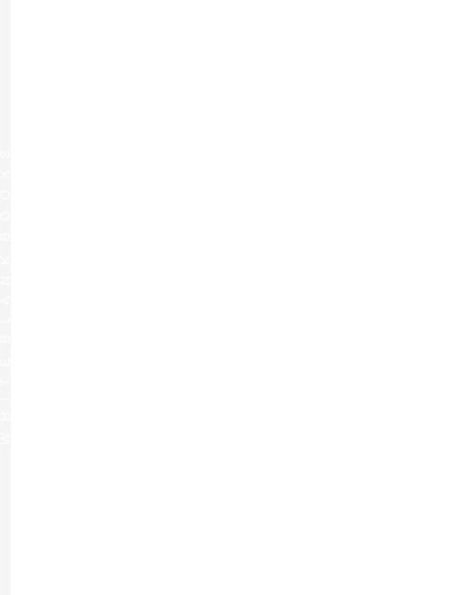
\includegraphics[height=0.2 \textheight]{Imagenes/vientoT}
		\caption{Dirección que el viento toma respecto al jugador.}
		\label{fig:vientoT}
	\end{figure}